%*
%* Seven Kingdoms: Ancient Adversaries
%*
%* Copyright 1997,1998 Enlight Software Ltd.
%* Copyright 2018 Timothy Rink
%*
%* This program is free software: you can redistribute it and/or modify
%* it under the terms of the GNU General Public License as published by
%* the Free Software Foundation, either version 2 of the License, or
%* (at your option) any later version.
%*
%* This program is distributed in the hope that it will be useful,
%* but WITHOUT ANY WARRANTY; without even the implied warranty of
%* MERCHANTABILITY or FITNESS FOR A PARTICULAR PURPOSE.  See the
%* GNU General Public License for more details.
%*
%* You should have received a copy of the GNU General Public License
%* along with this program.  If not, see <http://www.gnu.org/licenses/>.
%*
%*

\chapter{Mercanaries}

\section{Hiring Mercenaries and Skilled Foreign Workers}

\begin{wrapfigure}{l}{0.2\textwidth}
	\vspace{-20pt}
	\begin{center}
		
\includegraphics[width=0.2\textwidth]{Iinn}
		\\ Inn
	\end{center}
	\vspace{-20pt}
\end{wrapfigure}

Inns are gathering places used by travelers from around the area. Perhaps exiled from their homelands---or perhaps in search of adventure or gold, these travelers are a mixed bag of skilled mercenaries, accomplished artisans, and Spies.

Your Inns may be placed anywhere; they need not be Linked directly or indirectly with any other building.

\subsection{How to Hire a Mercenary}

A Mercenary is hired into your service by selecting the Inn and then scrolling down the list of people there. You will see their specialty as well as their level of skill and asking price.

\clearpage

To hire, \textbf{Click} on the person that you are interested in and then \textbf{Click} on the \textbf{Hire Tile} on the bottom left.

\begin{wrapfigure}{r}{0.5\textwidth}
	\vspace{-20pt}
	\begin{center}
		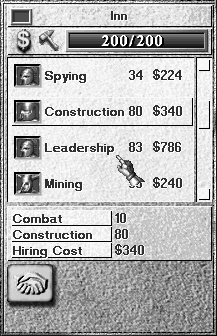
\includegraphics[width=0.4\textwidth]{Iinninfo}
	\end{center}
	\vspace{-20pt}
\end{wrapfigure}

These travelers will come and go from the Inn, so if you see nobody of use, make sure to come back later as there is a good chance that you will find what you seek.

It is important to remember that Mercenaries also tend to have a low level of loyalty to your rule. Incentives in the way of Grants or Honors may be called for to raise that level.

\clearpage

\subsection{When to Hire Mercenaries}

You will notice that you find more people at the Inns in the early years of the game. This reflects the fact that at that time, national allegiances are not well established. It is important, therefore, that you hire some of the best that you can find in the early years of the game.

As time goes on, you will find fewer and fewer good people to hire. You will instead have to concentrate on training your own.

\begin{center}
	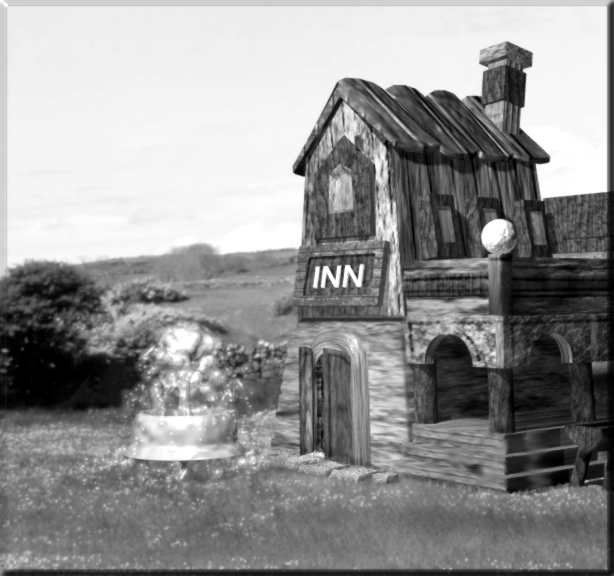
\includegraphics[width=0.7\linewidth]{Ainn}
\end{center}